\documentclass[addpoints,11pt]{exam}

\usepackage{alltt}
\usepackage[margin=1in]{geometry}   % set up margins
\usepackage[T1]{fontenc}
\usepackage[usenames,dvipsnames]{xcolor}
\usepackage{enumerate}              % fancy enumerate
\usepackage{amsmath}                % used for \eqref{} in this document
\usepackage{amsthm}
\theoremstyle{definition}
\newtheorem{exmp}{Example}[section]
\usepackage{verbatim}               % useful for \begin{comment} and \end{comment}
\usepackage{eurosym}                % used for euro symbol
\usepackage{caption} 
\usepackage{graphicx}
\graphicspath{{Figures/}}
\usepackage{subcaption}
\usepackage{color}
\usepackage{float}
\usepackage{amssymb}
\usepackage{sgamevar}
\usepackage{sgame}
\usepackage[colorlinks=true]{hyperref}
\hypersetup{colorlinks=true, citecolor=ForestGreen, linkcolor=BlueViolet, urlcolor=Magenta}



%Solutions or nah (blank next two lines out for no solutions, unblank #3)
%\printanswers
%\newcommand{\dd}[1]{\par {\textbf{\textcolor{red}{#1}}}}
\newcommand{\dd}[1]{}  


\setlength\parindent{0pt}
\unframedsolutions
\SolutionEmphasis{\color{red}}
\CorrectChoiceEmphasis{\color{red}}
\renewcommand{\choicelabel}{(\alph{choice})}
\newcommand{\blank}[0]{\underline{\hspace{3cm}}}
\pointformat{\bfseries[\thepoints]}
\pointpoints{pt}{pts}
\pointsinrightmargin

\begin{document}


	\title{\textbf{Problem Set 3 \dd{Answers and Selected Solutions}} \\ \vspace{2 mm} {\large Principles of Economics}}
	\author{David A. D\'iaz}
	\date{}
	\maketitle

\subsection*{The Costs of Production}

\begin{questions}
	
			\question AJ opens a lemonade stand for two hours. He spends \$10 for ingredients and sells \$60 worth of lemonade. In those same two hours, he could have cleaned his neighbor's pool for \$40. AJ has an accounting profit of \blank and an economic profit of \blank.
			
			\begin{choices}
				\CorrectChoice \$50; \$10
				\choice \$90; \$50
				\choice \$10; \$50
				\choice \$50; \$90
			\end{choices}
			
			\begin{solution}
				Total revenue = \$60. Explicit costs = \$10. Implicit costs = \$40. Accounting profit = TR -- explicit costs = \$50. Economic profit = TR -- (explicit costs + implicit costs) = \$10.
			\end{solution}
			
\question Ray left his job as a stock broker where he was earning \$70,000 a year to start a cookie business. Over the past year, Ray sold 50,000 boxes of cookies at a price of \$4.00 per box. He also incurred labor costs of \$60,000 and paid \$20,000 for raw materials. Ray's accounting profit for the year was

\begin{choices}
	\choice \$70,000.
	\CorrectChoice \$120,000.
	\choice \$50,000.
	\choice \$80,000.
\end{choices}

\question A firm is able to produce 165 units of output per day when 15 workers are hired. If the firm hires 16 workers, it can increase its output to 176 units. The marginal product of the 16th worker is

\begin{choices}
	\choice 10 units.
	\choice 16 units.
	\CorrectChoice 11 units.
	\choice 176 units.
\end{choices}
			
			\question A firm is producing 100 units with an average total cost of \$25 and a marginal cost of \$15. If it were to increase production to 101 units, which of the following must occur?
			
			\begin{choices}
				\choice Marginal cost would decrease.
				\choice Marginal cost would increase.
				\CorrectChoice Average total cost would decrease.
				\choice Average total cost would increase.
			\end{choices}
			
			\begin{solution}
				If $MC < ATC$, then it must be that $ATC$ are decreasing.
			\end{solution}
			
			\question Bluth's Bananas currently employs 5 workers and produces 1,000 frozen bananas a day. In preparation for the busy summer season, the firm is debating whether they should hire 5 more workers. If they do, they project they could produce 1,500 frozen bananas a day. Given this, the marginal product of labor per worker from these additional workers would be
			
			\begin{choices}
				\choice 1,500.
				\choice 500.
				\choice 150.
				\CorrectChoice 100.
			\end{choices}
			
			\begin{solution}
				$MP_L = \frac{\Delta Q}{\Delta L} = \frac{(1,500 - 1,000)}{5} = 100.$
			\end{solution}
			
\question Keystone Fireworks has fixed costs of \$10 and the marginal costs outlined in Table \ref{MC9}.

\begin{table}[H]
	\caption{Marginal Costs for Cheerwine}
	\label{MC9}
	\centering
	\begin{tabular}{  c| c}   
		Quantity & Marginal Cost\\
		\hline
		1 & \$2 \\
		2 & \$4 \\
		3 & \$7 \\
		4 & \$11 \\
		5 & \$16 \\
		6 & \$22 \\
	\end{tabular}
\end{table}

What is the average total cost of producing the fifth unit?

\begin{choices}
	\choice \$3.20
	\CorrectChoice \$10.00
	\choice \$5.20
	\choice \$8.00
\end{choices}
			
			\question Shell Tires has fixed costs of \$300,000 per year. Last year, it produced 10,000 tires with an average variable cost of \$80. What were the firm's average total costs for last year?
			
			\begin{choices}
				\choice \$80
				\choice \$90
				\choice \$100
				\CorrectChoice \$110
			\end{choices}
			
			\begin{solution}
				$ATC = TC/Q = (FC + VC)/Q = AFC + AVC = \$300,000/10,000 + \$80 = \$110$.
			\end{solution}
			
			\question Keystone Fireworks has fixed costs of \$100 and the marginal costs outlined in Table \ref{tab1}.
			
			\begin{table}[H]
				\caption{Marginal Costs for Keystone}
				\label{tab1}
				\centering
				\begin{tabular}{ c|c}      
					Quantity & Marginal Cost\\     
					\hline
					1 & \$2   \\
					2 & \$4   \\
					3 & \$6  \\
					4 & \$8   \\
					5 & \$10  \\
					6 & \$12  \\
				\end{tabular}
			\end{table}
			
			What is the average variable cost of producing the fifth unit?
			
			\begin{choices}
				\choice \$2
				\CorrectChoice \$6
				\choice \$10
				\choice \$30
			\end{choices}
			
			\begin{solution}
				At Q=0, VC = \$0. At Q=1, MC = \$2 which means VC increased by \$2 when going from Q=0 to Q=1. So, at Q=1, VC = \$2. At Q=2, MC = \$4, so VC increased by \$4 when going from Q=1 to Q=2. Since VC=\$2 at Q=1, at Q=2 VC =\$6. Continuing this process until Q=5, we have that VC = \$30. AVC = VC/Q = \$30/5 = \$6.
				
						\begin{table}[H]
							\caption{Marginal Costs for Keystone}
							\label{tab1}
							\centering
							%Change last column to "H" for solutions
							\begin{tabular}{ c|c| c}      
								Quantity & Marginal Cost & \dd{Variable Costs}\\     
								\hline
								1 & \$2 & \dd{\$2} \\
								2 & \$4 & \dd{\$6} \\
								3 & \$6 & \dd{\$12}\\
								4 & \$8 & \dd{\$20}  \\
								5 & \$10 & \dd{\$30} \\
								6 & \$12 & \dd{\$42}\\
							\end{tabular}
						\end{table}
						
			\end{solution}
			
			\question A firm currently produces 1,000 units of output with an average variable cost of \$5.10. The firm has fixed costs of \$5,000. If the firm were to produce 1,001 units, its total variable costs would be \$5,400. What is the marginal cost to the firm of producing 1,001 units?
			
			\begin{choices}
				\choice \$5,400
				\CorrectChoice \$300
				\choice \$5,100
				\choice \$400
			\end{choices}
			
			\dd{At 1,000 units, $VC = 1,000 \times 5.10 = \$5,100.$ $MC = \frac{\Delta VC}{\Delta Q} = \frac{(5,400 - 5,100)}{1} = \$300.$}
			
	\question A firm is producing 500 units with an average total cost of \$10 and a marginal cost of \$15. If it were to increase production to 501 units, which of the following must occur?
	
	\begin{choices}
		\choice Marginal cost would decrease.
		\choice Marginal cost would increase.
		\choice Average total cost would decrease.
		\CorrectChoice Average total cost would increase.
	\end{choices}
	
	
\question Jay's Chocolates produces boxes of chocolates for its mail order catalogue business. He rents a small room for \$150 a week that serves as his factory. Workers can be hired for \$275 per week. There are no other costs. 

Table \ref{jay} shows certain characteristics of the business. One week, Jay realizes revenue of \$1,100, leading to a profit of \$125. How many boxes of chocolate did he produce?

\begin{table}[H]
	\caption{Jay's Chocolate}
	\centering
	\begin{tabular}{ c|c|c|c|c|c}        
		
		Workers  & Boxes & MPL & Cost of Factory & Cost of Workers & Total Cost \\
		\hline
		0 & 0 & & & & \\
		1 & & 330 & 150 & 275 & 425 \\
		2 & 630 & &&& \\
		3 &  & 150 & & 825 & 975  \\
		4 & 890 & &&& \\
		5 & 950 & 60 & & 1,375 & \\
		6 &  & 10 &&& 1,800 \\
	\end{tabular}
	\label{jay}
\end{table}

\begin{choices}
	\choice 140
	\choice 330
	\CorrectChoice 780
	\choice 950
\end{choices}

\newpage

\question If there are no implicit costs of production,

\begin{choices}
	\choice economic profit will exceed accounting profit.
	\choice accounting profit will exceed economic profit.
	\CorrectChoice economic profit and accounting profit will be equal.
	\choice economic profit will be zero.
	\choice accounting profit will be zero.
\end{choices}

\question If a production function exhibits diminishing marginal product, its slope 

\begin{choices}
	\CorrectChoice becomes flatter as the quantity of input increases.
	\choice becomes steeper as the quantity of input increases.
	\choice is constant.
	\choice could be any of the above.
\end{choices}

\question Which of the following statements is true?

\begin{choices}
	\choice All costs are fixed in the long run.
	\CorrectChoice All costs are variable in the long run.
	\choice All costs are fixed in the short run.
	\choice All costs are variable in the short run.
\end{choices}

		\question Your roommate's food truck sells delicious burritos every Friday night. He tells you a story that as he closed up shop last weekend, an inebriated patron yelled at him to make him one for \$10.00. Your roommate had already sold 200 burritos that night, but usually has to sell them for \$4.00 due to market conditions. He tells you that he obviously sold him the burrito for \$10.00. If he faces the cost schedule detailed in Table \ref{tab5}, was this the right decision? Explain why or why not. 
		
		
		\begin{table}[H]
			\caption{Burrito Costs}
			\centering
			\begin{tabular}{ c|c}        
				
				Quantity  & ATC \\
				\hline
				199 & \$1.99 \\
				200 & \$2.00 \\
				201 & \$2.05 \\
			\end{tabular}
			\label{tab5}
		\end{table}
		
		\begin{solution}
			Your roommate should sell the burrito as long as $MR \ge MC$. $MR = \$4.$ At Q=200, $TC = \$2.00 \times 200 = \$400$ and at Q=201 $TC = \$2.05 \times 201 = \$412.05.$ $MC = 412.05 - 400 = \$12.05$. Your friend should not have the sold burrito for \$10, as he would actually decrease his profit for the day by \$2.05.
		\end{solution}

			
		\end{questions}
	
		
		\subsection*{Perfect Competition}
		
		\begin{questions}
			
	
			\question If a profit-maximizing competitive firm is producing a quantity at which marginal cost is between average variable cost and average total cost, it will
			
			\begin{choices}
				\CorrectChoice keep producing in the short run, but exit the market in the long run.
				\choice shut down in the short run, but return to production in the long run. 
				\choice shut down in the short run and exit in the long run.
				\choice keep producing in both the short run and the long run.
			\end{choices}
			
			\begin{solution}
				A competitive firm produces where $P = MC$. For prices where $AVC < P < ATC$, the firm produces in the short-run, but will shut down in the long-run.
			\end{solution}
			

\newpage
	
		
		\question Profit for a firm in a perfectly competitive market is positive whenever
		
		\begin{choices}
			\choice $P < ATC$.
			\choice  $P < MC$.
			\choice $P > MC$.
			\CorrectChoice $P >ATC$.
		\end{choices}
		
		\begin{solution}
			$\Pi = TR - TC  = (P - ATC)\cdot Q \Rightarrow \Pi >0 \iff P > ATC$.
		\end{solution}
	
		\question Consultants hired by Sunnyside Eggs find that the firm has total fixed costs of \$50,000, total variable costs of \$25,000, and total revenues of \$40,000. Given this, in the short run the firm should \blank and make \blank profit.
		
		\begin{choices}
			\choice shut down; negative
			\choice shut down; zero
			\CorrectChoice stay open; negative
			\choice stay open; positive
		\end{choices}
	
			
		\begin{solution}
			Short-run decision: Shut down if $TR<VC$, operate if $TR>VC$. Firm should operate in the short run. $\Pi = TR - TC = \$40,000 - (50,000 + 25,000) = -\$35,000.$
		\end{solution}
		
\question The market for Kale is perfectly competitive. It follows that the demand for any individual soybean producer's output is 

\begin{choices}
	\choice perfectly inelastic.
	\CorrectChoice perfectly elastic.
	\choice unit elastic.
	\choice downward sloping.
\end{choices}

\question A firm in a perfectly competitive market sells 8 units of output and has a marginal revenue of \$8. What would be the firm's total revenue if it sold 4 units of output?

\begin{choices}
	\choice \$4
	\choice \$8
	\CorrectChoice \$32
	\choice \$64
	\choice There is not enough information to answer this question.
\end{choices}
		
\uplevel{For questions \ref{blah1} and \ref{blah2}, refer to Table \ref{tab2}.}
				\begin{table}[H]
							\centering
							\caption{Competitive Firm}
							\label{tab2}
							%Change to H's for HW
							\begin{tabular}{ c|c|c}        
								
								Quantity & Total Revenue & Total Cost  \\
								\hline
								0 & \$0  & \$30 \\
								1 & \$80 & \$50 \\
								2 & \$160 & \$80 \\
								3 & \$240 & \$120 \\
								4 & \$320 & \$170  \\
								5 & \$400 & \$230 \\
								6 & \$480 & \$300  \\
								7 & \$560 & \$380 \\
								8 & \$640 & \$470   \\
							\end{tabular}
						\end{table} 
						
\newpage

			
			\question \label{blah1} What is the marginal cost at the profit maximizing quantity?
			\begin{choices}
				\choice \$50
				\CorrectChoice \$80
				\choice \$230
				\choice \$300
			\end{choices}
			
			\begin{solution}
				Maximize profit at $Q$ where $MR = MC.$
			\end{solution}
			
			\question \label{blah2} What is the average fixed cost at the profit maximizing quantity?
			
			\begin{choices}
				\choice \$54.30
				\CorrectChoice \$4.28
				\choice \$50
				\choice \$80
			\end{choices}
			
			\begin{solution}
				$Q^* = 7$ (where $MR = MC).$ $FC = \$30$ (total cost at $Q=0$). $AFC = FC/Q = \$30/7 = \$4.28$.
			\end{solution}
			
	\question Suppose the market for corn is perfectly competitive. Which of the following represents the long-run relationship between the price, marginal cost, and average total cost at the profit-maximizing quantity?
	
	\begin{choices}
		\choice $P > MC = ATC$
		\choice $P = MC > ATC$ 
		\CorrectChoice $P = MC = ATC$
		\choice $P > MC > ATC$
	\end{choices}
			
			
			\question Natalie the baker wants to establish a pie factory in a competitive market. The cost of leasing the factory is \$800 a day. The profit maximizing quantity of pies is 1,000 a day, each pie sells for \$3, and has a variable cost of only \$1.50. Which of the following is true?
			
			\begin{choices}
				\CorrectChoice Natalie should enter the industry.
				\choice Natalie should not enter the industry.
				\choice Natalie would enjoy profits of \$3,000 a day.
				\choice Both (a) and (c) are true.
			\end{choices}
			
			\begin{solution}
				Enter market if $TR \ge TC \iff P \ge ATC$. $TR = \$3\cdot 1,000 = \$3,000$ and $TC = \$800 + \$1.50\cdot 1,000 = \$2,300$. Thus, Natalie should enter the market and will make a profit of $\$3,000 - \$2,300 = \$700/\text{day}.$
			\end{solution}
			
			\question In order to maximize profit, a firm in a perfectly competitive market will produce at the quantity where
			
			\begin{choices}
				\CorrectChoice $AR = MC$.
				\choice $P = ATC$.
				\choice $P = AVC$.
				\choice $MR = ATC$.
			\end{choices}

	\begin{solution}
		Always produce where $MR = MC$. For competitive firms, $MR = P = AR$.
	\end{solution}
	
		\question Suppose the market for corn is perfectly competitive. Which of the following represents the long-run relationship between the price, marginal cost, and average total cost at the profit-maximizing quantity?
		
		\begin{choices}
			\choice $P > MC = ATC$
			\choice $P = MC > ATC$ 
			\CorrectChoice $P = MC = ATC$
			\choice $P > MC > ATC$
		\end{choices}
		
		\begin{solution}
			Firms in PC produce where $P = MC$. In the long run, firms in PC make zero economic profit so $P=ATC$.
		\end{solution}

	\question Al's Burgers is a firm in a competitive market and faces the cost structure shown in Figure \ref{MC28}.
				
				\begin{figure}[H]
					\centering
					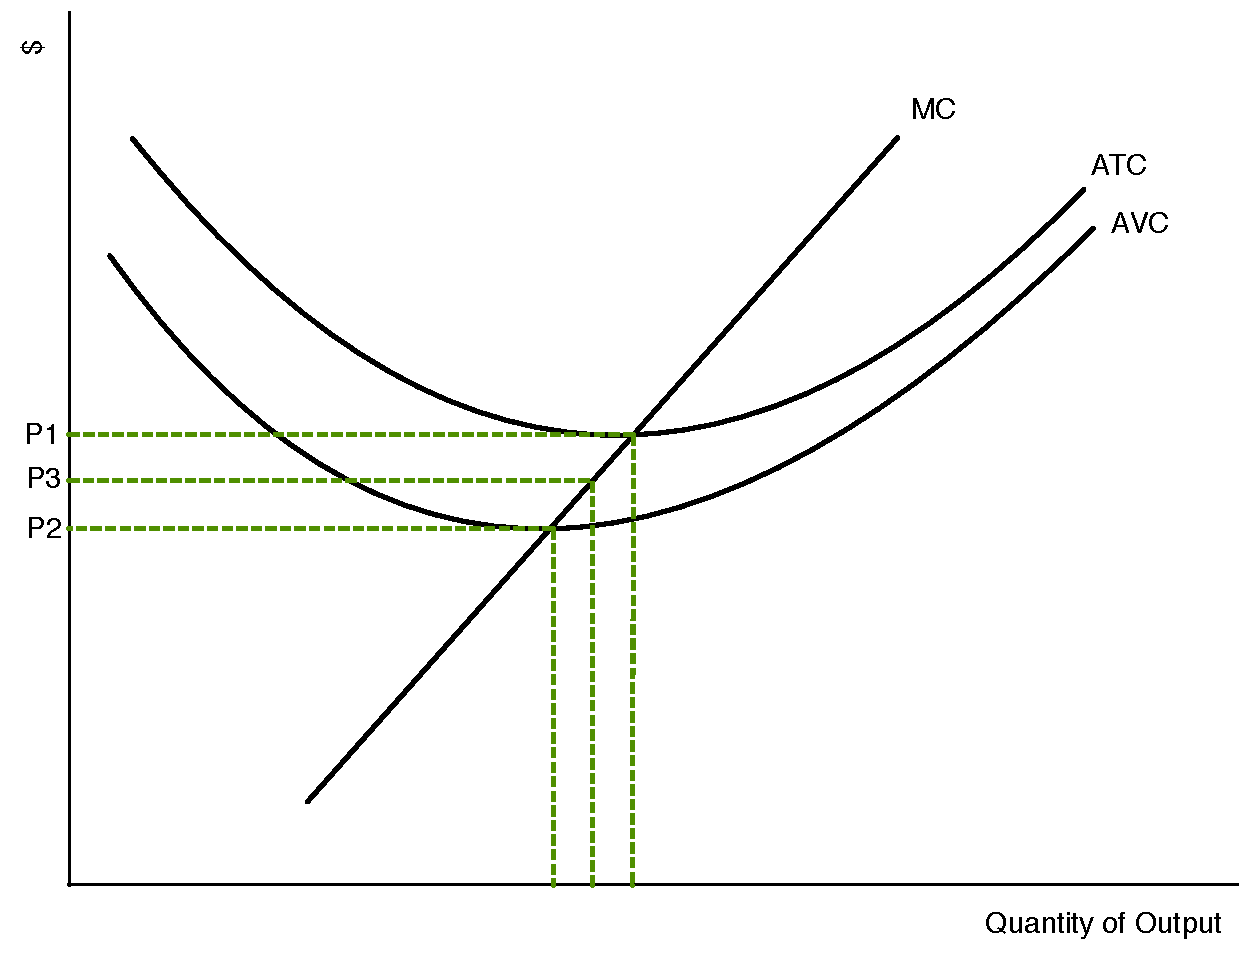
\includegraphics[scale=.45]{Exam1_MC27.pdf}
					\caption{Al's Burgers}
					\label{MC28}
				\end{figure}
				
				The firm decides to operate in the short run, but incurs economic losses. Thus, the market price must be 
				
				\begin{choices}
					\choice less than P2.
					\choice greater than P2 but less than P3.
					\choice greater than P3 but less than P1.
					\CorrectChoice greater than P2 but less than P1.
					\choice greater than P1.
				\end{choices}
				
			\begin{solution}
				Operate in SR along $MC$ curve above $AVC$. If operating at a loss, $P<ATC$ and so price must be $P2 < P < P1$.
			\end{solution}
				
\question In the short run, the competitive firm's supply curve is the 

\begin{choices}
	\choice entire marginal cost curve.
	\choice portion of the marginal cost curve that lies above the average total cost curve.
	\CorrectChoice portion of the marginal cost curve that lies above the average variable cost curve.
	\choice upward-sloping portion of the average total cost curve.
	\choice downward-sloping portion of the average total cost curve.
\end{choices}

\question A grocery store should close at night if the

\begin{choices}
	\choice total costs of staying open exceed the total revenue from staying open.
	\choice total revenue from staying open exceed the total costs of staying open.
	\CorrectChoice variable costs of staying open exceed the total revenue from staying open.
	\choice total revenue from staying open exceed the variable costs of staying open.
\end{choices}

\newpage

\question In the long run, firms will exit the market if the price of a good is less than 

\begin{choices}
	\choice marginal revenue.
	\choice marginal cost.
	\choice average revenue.
	\choice average variable cost.
	\CorrectChoice average total cost.
\end{choices}
	
	\question Natalie's Ball Bearings, Inc. faces the following costs of production outlined in Table \ref{tab4}.
	
	\begin{table}[h]
		\centering
		\caption{Cost of Ball Bearings}
		\label{tab4}
		\begin{tabular}{  c|c|c}        
			
			Quantity (in cases) & Total Fixed Costs & Total Variable Costs \\
			\hline
			0 & \$100  &  \\
			1 &  & \$50 \\
			2 &  & \$70 \\
			3 &  & \$90  \\
			4 &  & \$140 \\
			5 &  & \$200 \\
			6 &  & \$360  \\
		\end{tabular}
	\end{table} 
	
	\begin{parts}
		\part Suppose the market for ball bearings is perfectly competitive and the price of a case is \$50. The CEO sees that he can't make a profit, and so decides to shut down operations. What is the firm's profit (or loss) as a result of this decision? Do you agree with the CEO's decision? Why or why not? 
		
		\begin{solution}
			If firm shuts down, $TR$ = 0, $VC$ = 0, and $FC$ = \$100 so $\Pi = -\$100$. \\
			To find optimal quantity, use variable cost column to compute $MC$. $MC$ = \$50 at $Q=1$ and $Q=4$. At $Q=1$, $\Pi = \$50 \times 1 - \$150 = -\$100$. At $Q=4$, $\Pi = \$50 \times 4 - \$240 = -\$40$. Don't agree since $TR > VC$ at $Q=4$, the firm should produce in the SR even if it is making losses since it would lose more by shutting down.
		\end{solution}
		
		\part If instead the CEO decided to produce 1 case of ball bearings, what would be the firm's profit (or loss)? Is this the best decision? Why? 
		
		\begin{solution}
			See (a). Always produce on part of $MC$ curve past its minimum. $MC$ decreases from $Q=1$ to $Q=2$, so $Q=1$ cannot be optimal quantity.
		\end{solution}
	\end{parts}
	
	\question A firm is currently in a market with the conditions outlined in Table \ref{SA3}. The firm has fixed costs of \$1,500 per day.
	
	\begin{table}[H]
		\caption{Market Environment}
		\centering
		\begin{tabular}{c|c|c|c|c} 
			
			Quantity/day   & Total Revenue &  Marginal Cost & Variable Costs & Total Costs\\
			\hline
			1 & \$600 &  \$1,000 & \dd{1000} & \dd{2500}  \\
			2 & \$1,200 & \$400 & \dd{1400}  & \dd{2900} \\
			3 & \$1,800 & \$500 & \dd{1900}  & \dd{3400}  \\
			4 & \$2,400 & \$600 & \dd{2500} & \dd{4000} \\
			5  & \$3,000 & \$800 & \dd{3300}  & \dd{4800} \\
		\end{tabular}
		\label{SA3}
	\end{table}
	
	Use this information to answer the following questions.
	
	\begin{parts}
		\part What type of market environment is this firm in? Explain why. 
		
		\begin{solution}
			The firm is in a perfectly competitive market since $P = MR = \$600$.
		\end{solution}
		
		\part Fill in the column labeled ``Variable Costs.'' 
	
		
		\part Fill in the column labeled ``Total Costs.'' 
		
		\part What level of production should the firm operate at? Explain why.
		
		\begin{solution}
			The firm should operate at $Q^* = 0$ (shutdown) because $VC > TR$ at the quantity where $MR = MC$ ($Q=4$).
		\end{solution}
		
		\part What will be the firm's profits per day at this production level?
		
		\begin{solution}
			$\Pi = -\$1,500$ (fixed costs).
		\end{solution}
	\end{parts}
	
\end{questions}

\subsection*{Monopoly}

\begin{questions}

			\question Assuming the same cost structure, a competitive market produces \blank output at \blank prices than a monopoly market.
			
			\begin{choices}
				\choice less; lower
				\CorrectChoice more; lower
				\choice less; higher
				\choice more; higher
			\end{choices}
			
			\begin{solution}
				Monopolies charge a mark-up over the marginal cost and produce less than a competitive market.
			\end{solution}


		
\uplevel{Refer to Table \ref{tab3} for questions \ref{blah3} and \ref{blah4}.} 

		\begin{table}[h!]
			\caption{Monopolist Environment}
			\label{tab3}
			\centering
			\begin{tabular}{  c|c|c}    
				Price & Quantity Demanded & Total Cost \\    
				\hline
				\$170 & 0 & \$100 \\
				\$160 & 1 & \$140 \\
				\$150 & 2 & \$184 \\
				\$140 & 3 & \$230 \\
				\$130 & 4 & \$280 \\
				\$120 & 5 & \$335 \\
				\$110 & 6 & \$395 \\
				\$100 & 7 & \$475 \\ 
				\$90 & 8 & \$565 \\
			\end{tabular}
		\end{table}

			
			\question \label{blah3} What is the marginal cost of the 6$^{th}$ shirt?
			
			\begin{choices}
				\choice \$44
				\choice  \$46
				\choice  \$55
				\CorrectChoice \$60
			\end{choices}
			
			\begin{solution}
				$MC = \Delta TC/ \Delta Q$. At $Q=6$, $MC = 395 - 335 = \$60.$
			\end{solution}
			

			\question \label{blah4} What is total profit at the profit-maximizing quantity?
			
			\begin{choices}
				\choice \$100
				\choice \$245
				\CorrectChoice \$265
				\choice \$395
			\end{choices}
			
			\begin{solution}
				Maximize profit where $MC = MR$. $MR = \Delta TR/\Delta Q$, so need to find $TR = P\times Q$ at each price first, then find $MR$. $MR$ = $MC$ = \$60 at $Q=6$, so $Q^* =6$ and $\Pi = \$660 - 395 = \$265$.
			\end{solution}
			
\question Consider Table \ref{Mc}, which shows the environment faced by a monopolist.


\begin{table}[H]
	\caption{Market Environment}
	\label{Mc}
	\centering
	\begin{tabular}{  c| c | c }   
		Output & Total Revenue &  Variable Costs \\     
		\hline
		1 & \$50 & \$30 \\
		2 & \$80 & \$60 \\
		3 & \$90 & \$90 \\
		4 & \$80 & \$120  \\
		5 & \$50& \$150 \\
		6 & \$20& \$180 \\
		7 & \$10 & \$210 \\
	\end{tabular}
\end{table}

What price will this firm charge in order to maximize profits?

\begin{choices}
	\CorrectChoice \$40
	\choice \$30
	\choice \$20
	\choice \$10
\end{choices}


\uplevel{Use Figure \ref{MC10}, which represents the environment faced by a monopoly, for questions \ref{blah5} and \ref{blah6}.}

\begin{figure}[H]
	\centering
	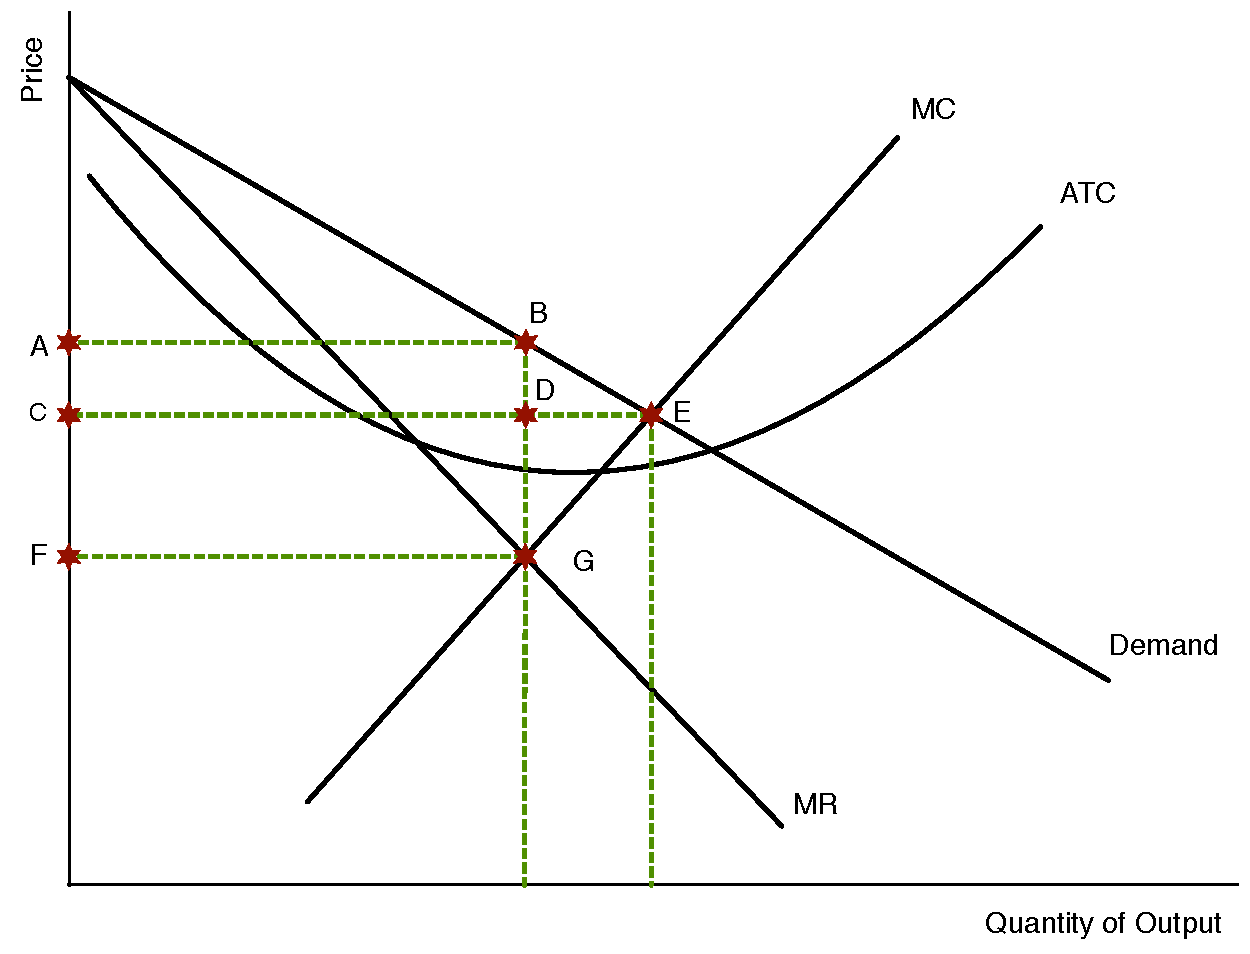
\includegraphics[scale=.4]{Exam2_MC10.pdf}
	\caption{Monopolist Environment}
	\label{MC10}
\end{figure}


	\question \label{blah5} Which of the following represents the lost trade that is responsible for the deadweight loss?
	
	\begin{choices}
		\choice Distance ab
		\choice Distance ce
		\CorrectChoice Distance de
		\choice Distance cd
	\end{choices}
	
	\begin{solution}
		Optimal quantity where $MC$ = Demand. Monopolist produces where $MR = MC$. Lost trades between distance de.
	\end{solution}
	
	\question \label{blah6} Which of the following areas represents the deadweight loss due to monopoly pricing?
	
	\begin{choices}
		\CorrectChoice Triangle bge
		\choice Triangle bde
		\choice Rectangle acdb
		\choice Rectangle cfgd
	\end{choices}
	
	\begin{solution}
		DWL comes from those trades that are not taking place where demand is above $MC$.
	\end{solution}
	
	
\question Which of the following is \textbf{not} a barrier to entry in a monopolized market?

\begin{choices}
	\choice The government gives a single firm the exclusive right to produce some good.
	\choice The costs of production make a single producer more efficient than a large number of producers.
	\choice A key resource is owned by a single firm.
	\CorrectChoice A single firm is very large.
\end{choices}

\question A firm whose average total cost continually declines at least to the quantity that will supply the entire market is known as a 

\begin{choices}
	\choice perfect competitor.
	\CorrectChoice natural monopoly.
	\choice government monopoly.
	\choice regulated monopoly.
\end{choices}	

\question Which of the following statements about price and marginal revenue in competitive and monopolized markets is true?

\begin{choices}
	\choice Price equals marginal revenue in both markets.
	\CorrectChoice Price equals marginal revenue in competitive markets, while price exceeds marginal revenue in monopoly markets.
	\choice Price exceeds marginal revenue in competitive markets, while price equals marginal revenue in monopoly markets.
	\choice Price exceeds marginal revenue in both markets.
\end{choices}
	
\question Consider Figure \ref{MC35}, which shows the cost structure of a monopolist.


\begin{figure}[H]
	\centering
	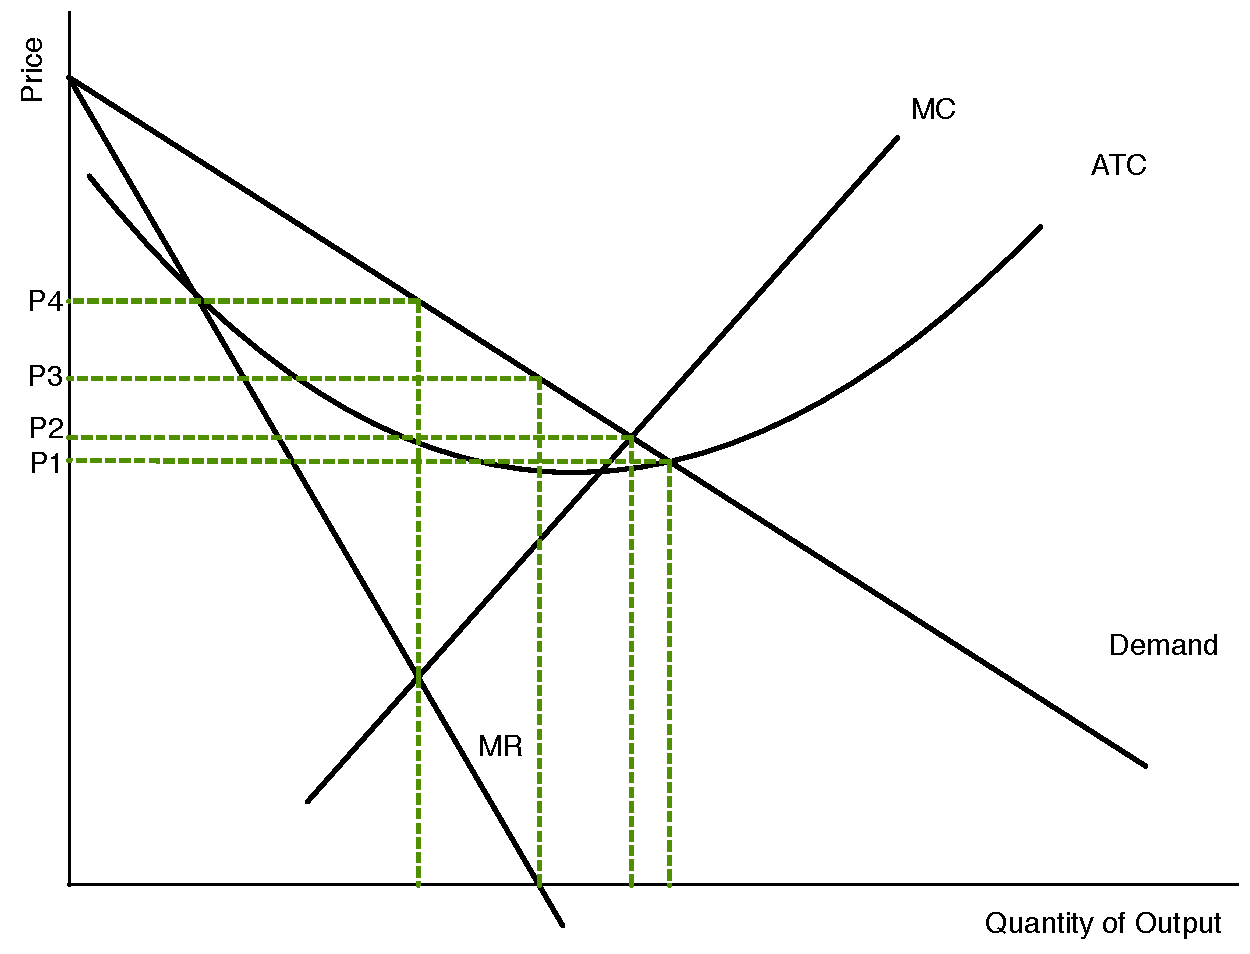
\includegraphics[scale=.40]{Final_MC35.pdf}
	\caption{Monopolist Environment}
	\label{MC35}
\end{figure}

If the firm wishes to maximize total revenue, it should charge price \underline{\hspace{3cm}}, while the price it should charge to maximize output while not making losses is \underline{\hspace{3cm}}.

\begin{choices}
	\choice P4; P2
	\CorrectChoice P3; P1
	\choice P2; P4
	\choice P3; P2
	\choice None of the above
\end{choices}

\begin{solution}
	Maximize $TR$ where at $Q$ where $MR = 0$. Trace up to demand curve to find price ($P3$). Losses occur when $P<ATC$. Lower price until $P=ATC$ to maximize output while not making losses. $P = P1$.
\end{solution}

\newpage

	\question A profit-maximizing monopolist will produce the level of output at which
	
	\begin{choices}
		\choice average revenue is equal to average total cost.
		\choice price is equal to marginal cost.
		\CorrectChoice marginal revenue is equal to marginal cost.
		\choice total revenue is equal to opportunity cost.
	\end{choices}
	
	\begin{solution}
		Any firm should produce where $MR = MC$ in order to maximize profits. This holds true in any type of market structure. (b) is only true for firms in a perfectly competitive market.
	\end{solution}
	
	
	\question If economies of scale exist, and government regulators force the monopolist to set price equal to marginal cost,
	
	\begin{choices}
		\choice the monopolist will still earn a profit, just smaller than with no regulation.
		\choice there will be no incentive to innovate.
		\choice the market will be less efficient than if regulators set prices equal to average total cost.
		\CorrectChoice the monopolist will be taking a loss.
	\end{choices}
	
	\begin{solution}
		For monopolies with economies of scale, $MC < ATC$. If the government forces the monopolist to charge $P=MC$ (this is the point where the demand and MC curve meet), then $P<ATC$ and $\Pi <0$.
	\end{solution}
	
\question Suppose a firm sells 25 units at a price of \$10. Calculate its marginal revenue per unit of output if it sells 5 more units of output when it reduces its price to \$9. Is this firm in a  competitive market or non-competitive market?

\begin{choices}
	\choice \$20; non-competitive
	\CorrectChoice \$4; non-competitive
	\choice \$270; non-competitive
	\choice \$2.50; competitive
	\choice None of the above.
\end{choices}

\question Using government regulations to force a natural monopoly to charge a price equal to its marginal cost will

\begin{choices}
	\choice improve efficiency.
	\choice raise the price of the good.
	\choice attract additional firms to the market.
	\CorrectChoice cause the monopolist to exit the market.
\end{choices}

\question Which of the following statements about price discrimination is \textbf{not} true?

\begin{choices}
	\choice Price discrimination can raise economic welfare.
	\choice Price discrimination requires that the seller be able to separate buyers according to their willingness to pay.
	\CorrectChoice Perfect price discrimination generates a deadweight loss.
	\choice Price discrimination increases a monopolist's profits.
\end{choices}

\newpage

\question Suppose a firm has a patent on a process to make unique smoked salmon. Table \ref{tab} shows information about the demand curve facing this firm.

	\begin{table}[H]
		\caption{Demand for Smoked Salmon}
		\label{tab}
		\centering
		\begin{tabular}{  c|c}    
			Price & Quantity Demanded (lbs) \\    
			\hline
			\$20 & 0  \\
			\$18 & 1  \\
			\$16 & 2  \\
			\$14 & 3  \\
			\$12 & 4  \\
			\$10 & 5  \\
			\$8 & 6  \\
			\$6 & 7  \\
			\end{tabular}
			\end{table}
			
			
\begin{parts}
	\part Suppose there are no fixed costs to produce this salmon and that the marginal cost of production is a constant \$6 per pound. Note: This implies that the average total cost is also a constant \$6 per pound. What is the quantity and price chosen by the monopolist?
	\begin{solution}
		The monopolist should produce at the quantity were $MR = MC$ (or as close as possible such that $MR > MC$). From the table, we need to find the marginal revenue from each pound of salmon:
	\begin{table}[H]
			\caption{Demand for Smoked Salmon}
			\label{tab10}
			\centering
			\begin{tabular}{  c|c | c | c}    
				Price & Quantity Demanded (lbs) & TR ($P\times Q)$ & MR ($\Delta TR/\Delta Q$) \\    
				\hline
				\$20 & 0 & 0 & --- \\
				\$18 & 1 & 18 & 18 \\
				\$16 & 2 & 32 & 14  \\
				\$14 & 3 & 42 & 10  \\
				\$12 & 4 & 48 & 6 \\
				\$10 & 5 & 50 & 2  \\
				\$8 & 6 & 48 & $-2$ \\
				\$6 & 7 & 42 & $-6$  \\
			\end{tabular}
		\end{table}		
	Thus, the monopolist should produce 4 units. The corresponding price is \$12.
	\end{solution}
	\part What is the monopolist's profit at this quantity?
	\begin{solution}
		$\Pi = (P - ATC) \times Q = (\$12 - \$6) \times 4 = \$24$.
	\end{solution}
	\part What is the price and quantity that maximizes total surplus?
	\begin{solution}
		The efficient quantity (where total surplus is maximized) is where $P = MC$. 
		This corresponds to a price of \$6 and a quantity of 7 units.
	\end{solution}
	\part Compare the monopoly and the efficient solution. Is the monopolist's price too high or too low? Is the monopolist's quantity too high or too low?
	\begin{solution}
		As usual, the monopolist charges a higher pricer and produces less than the optimal quantity.
	\end{solution}
	\part What is the deadweight loss in this market if the monopolist charges the monopoly price?
	\begin{solution}
		The deadweight loss in a monopoly market comes from the unrealized transactions where the buyer value exceeds the marginal cost of production. In problem, only 4 lbs of salmon are produced by the monopolist, but the efficient quantity is 7 lbs. The deadweight loss is the difference between the buyer value and marginal cost for the transactions not taking place. $DWL = (\$12 - \$6) + (\$10 - \$6) + (\$8 - \$6) + (\$6 - \$6) = \$12$.
	\end{solution}
	\part If the monopolist is able to perfectly price discriminate without cost, is the outcome efficient? What is the value of total surplus in this case?
	\begin{solution}
		Yes, this would be efficient. In this case, the monopolist would charge each consumer who is willing to pay above the marginal cost exactly their willingness to pay. Thus, consumer surplus is zero and the producer surplus is equal to the total surplus. The surplus realized from each transaction for the monopolist is the consumer's willingness to pay (i.e., the price they pay) and the marginal cost. $TS = PS = (\$20 - \$6) + (\$18 - \$6) + (\$16 - \$6) + (\$14 - \$6) + (\$12 - \$6) + (\$10 - \$6) + (\$8 - \$6) + (\$6 - \$6) = \$56$.
	\end{solution}
\end{parts}


\end{questions}




\end{document}